\chapter{Taxonomy of high-level SAF microarchitecture blocks (FMT,SKIP)}
\label{chapter:saf_microarchitectures}

%This chapter will introduce

%\begin{itemize}
%    \item A taxonomy of high-level SAF microarchitecture blocks %(FMT, SKIP)
%    \item A scheme for ``concretizing'' Sparseloop-style SAFs (which are purely declarative) into high-level SAF microarchitecture blocks.
%\end{itemize}

%\section{SAF microarchitectures}
%\label{chapter:saf_microarchitectures_section}

This section will overview the taxonomy of high-level SAF microarchitecture blocks considered in this work. As described in Section~\ref{chapter:conceptual_framework}, the highest level of SAF microarchitecture abstraction consists of abstract FMT (format microarchitecture) and SKIP (skipping microarchitecture) blocks which represent SAF microarchitectures in the most format- and context-agnostic manner possible.

Modeled off of Accelergy\cite{accelergy}, the high-level format-agnostic SKIP and FMT blocks are ``compound components'', i.e. high-level components assembled from lower-level components; in this case, high-level SAF microarchitecture blocks are assembled from SAF microarchitecture \textit{primitives} (Section~\ref{chapter:primitive_taxo_model}) connected together by wires. These two layers of abstraction, provide an easy way to move between high-level format- and context-agnostic representations, and lower-level representations that are co-designed for representation format and other surrounding design considerations.

Like SAF microarchitecture primitives, high-level SAF microarchitecture blocks have taxonomic attributes, as well as a list of supported customizations. Unlike SAF microarchitecture primitives, high-level microarchitecture blocks are not associated with RTL blocks or analytical models: a high-level SAF microarchitectural block derives its area and action energy from its SAF microarchitecture primitive subcomponents. 

Each supported customization is associated with (1) a different set of SAF microarchitecture primitives, and (2) a different topology for wiring the primitives together.

The particular customization cannot be determined unless all attributes of the high-level SAF microarchitecture block have been specified. However, the implementation topology associated with a particular customization, may itself have some primitives with unspecified attributes. These unspecified primitive attributes within a high-level SAF microarchitecture primitive topology, are referred to as ``free parameters'', and they represent design decisions which are not constrained by the representation format or other surrounding design characteristics. The user is free to adjust these free parameter attributes as part of design-space exploration.

\section{Format microarchitectures}

Format microarchitectures (FMT blocks) are introduced in Section~\ref{chapter:conceptual_framework}; the function of FMT blocks is to facilitate pipelined fibertree metadata parsing, traversal, and (when required) computing explicit coordinates to support coordinate arithmetic. See Figure~\ref{fig:FMT}.

\begin{figure}[H]
    \centering
    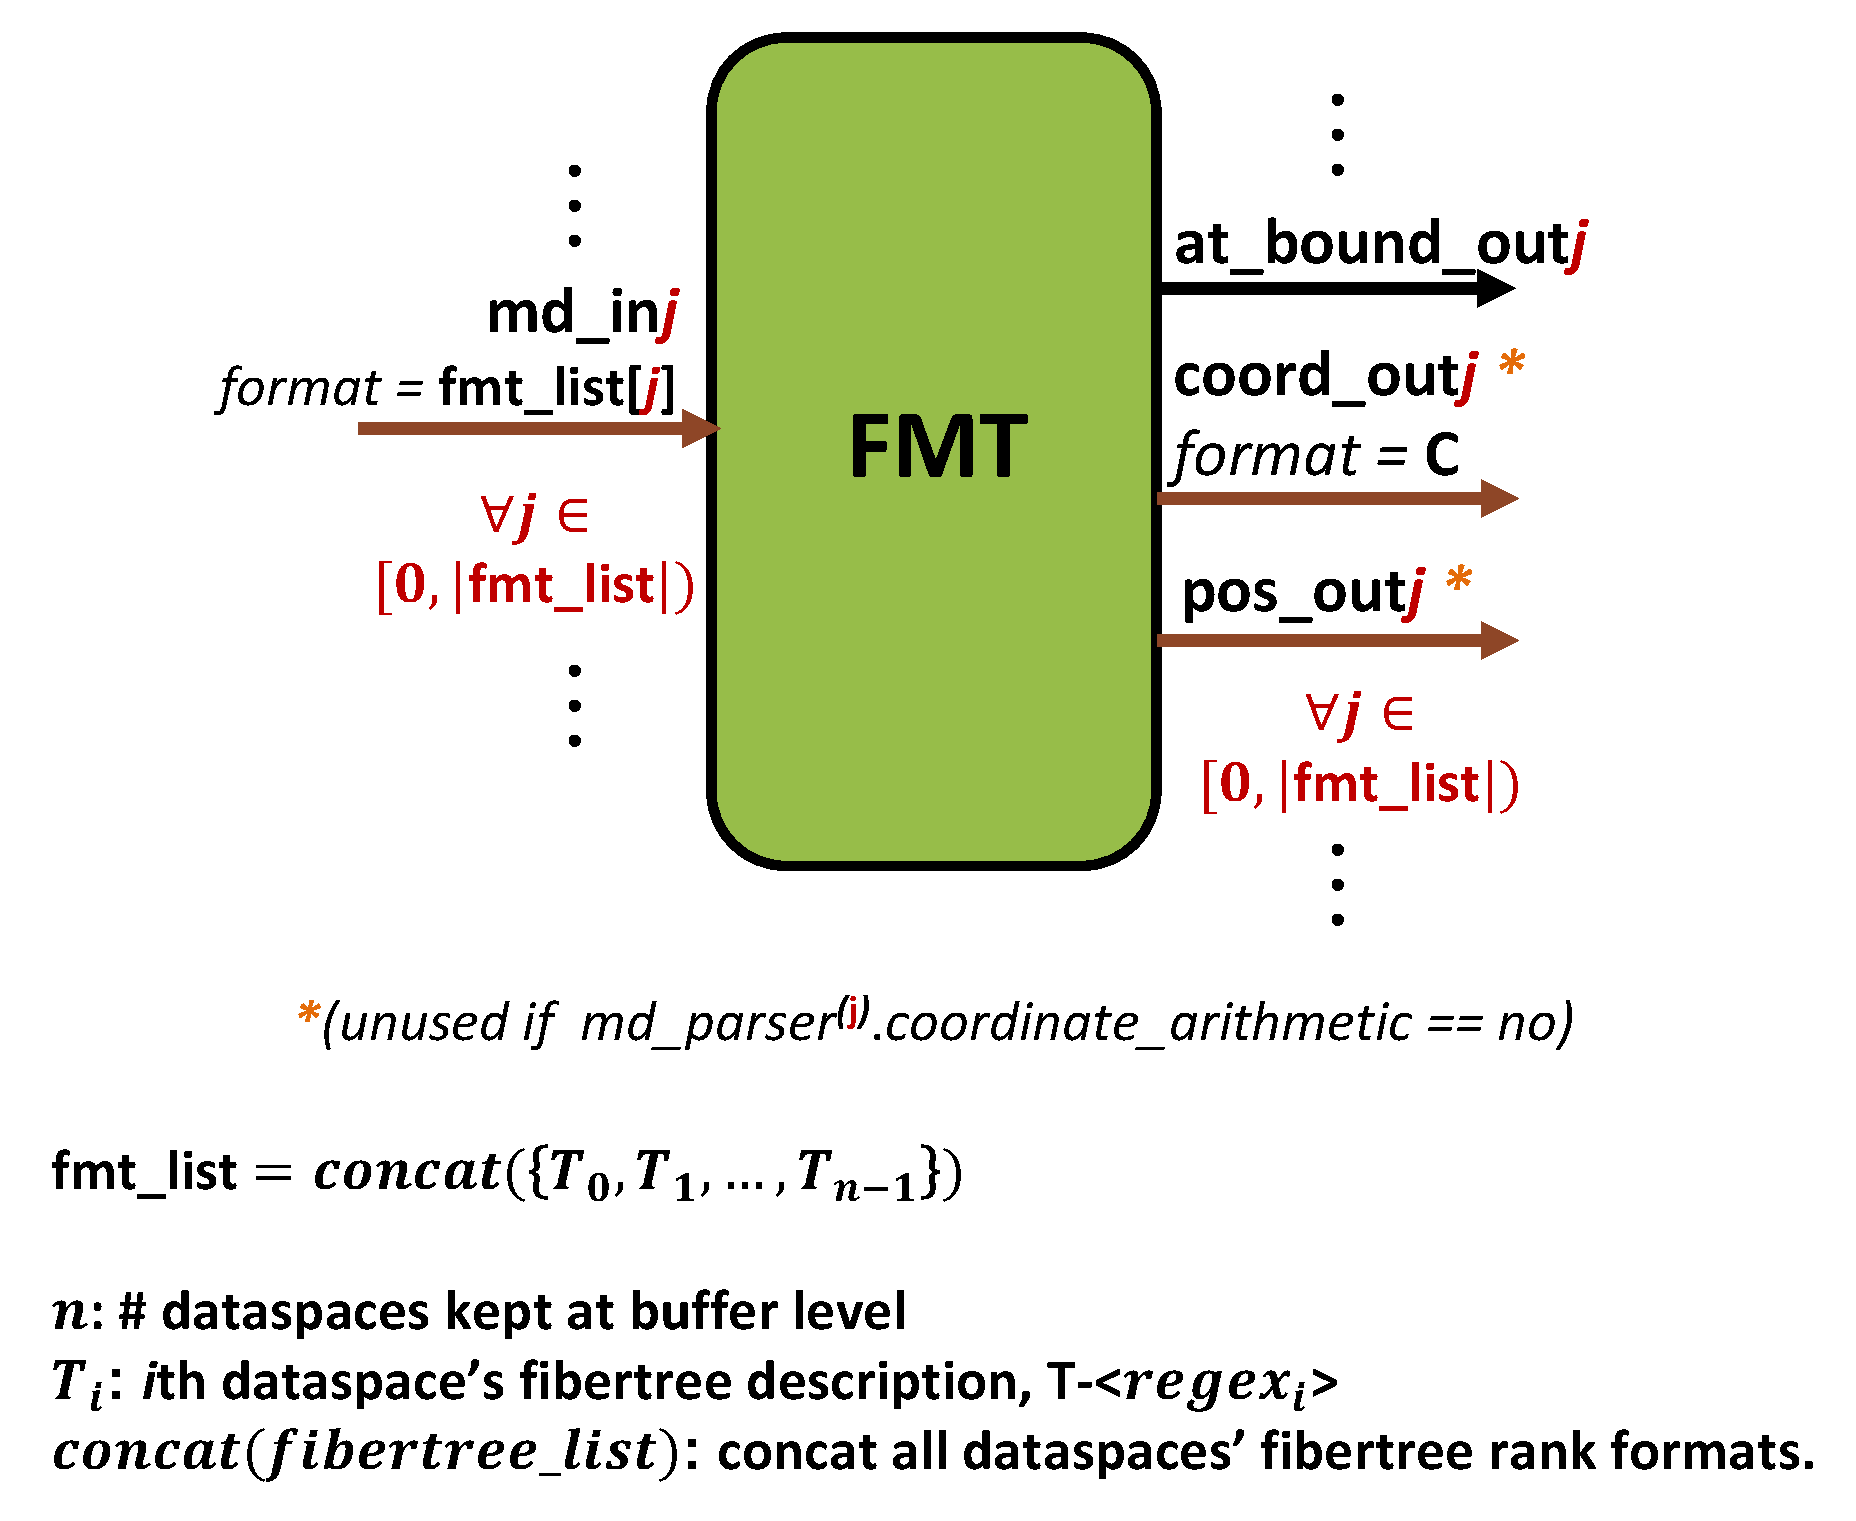
\includegraphics[width=0.95\textwidth]{figures/FMT.pdf}
    \caption{Format microarchitecture compound component (FMT block) category template. If an architectural buffer has a format SAF, a format microarchitecture must be bound to it.}
    \label{fig:FMT}
\end{figure}

\begin{figure}[H]
    \centering
    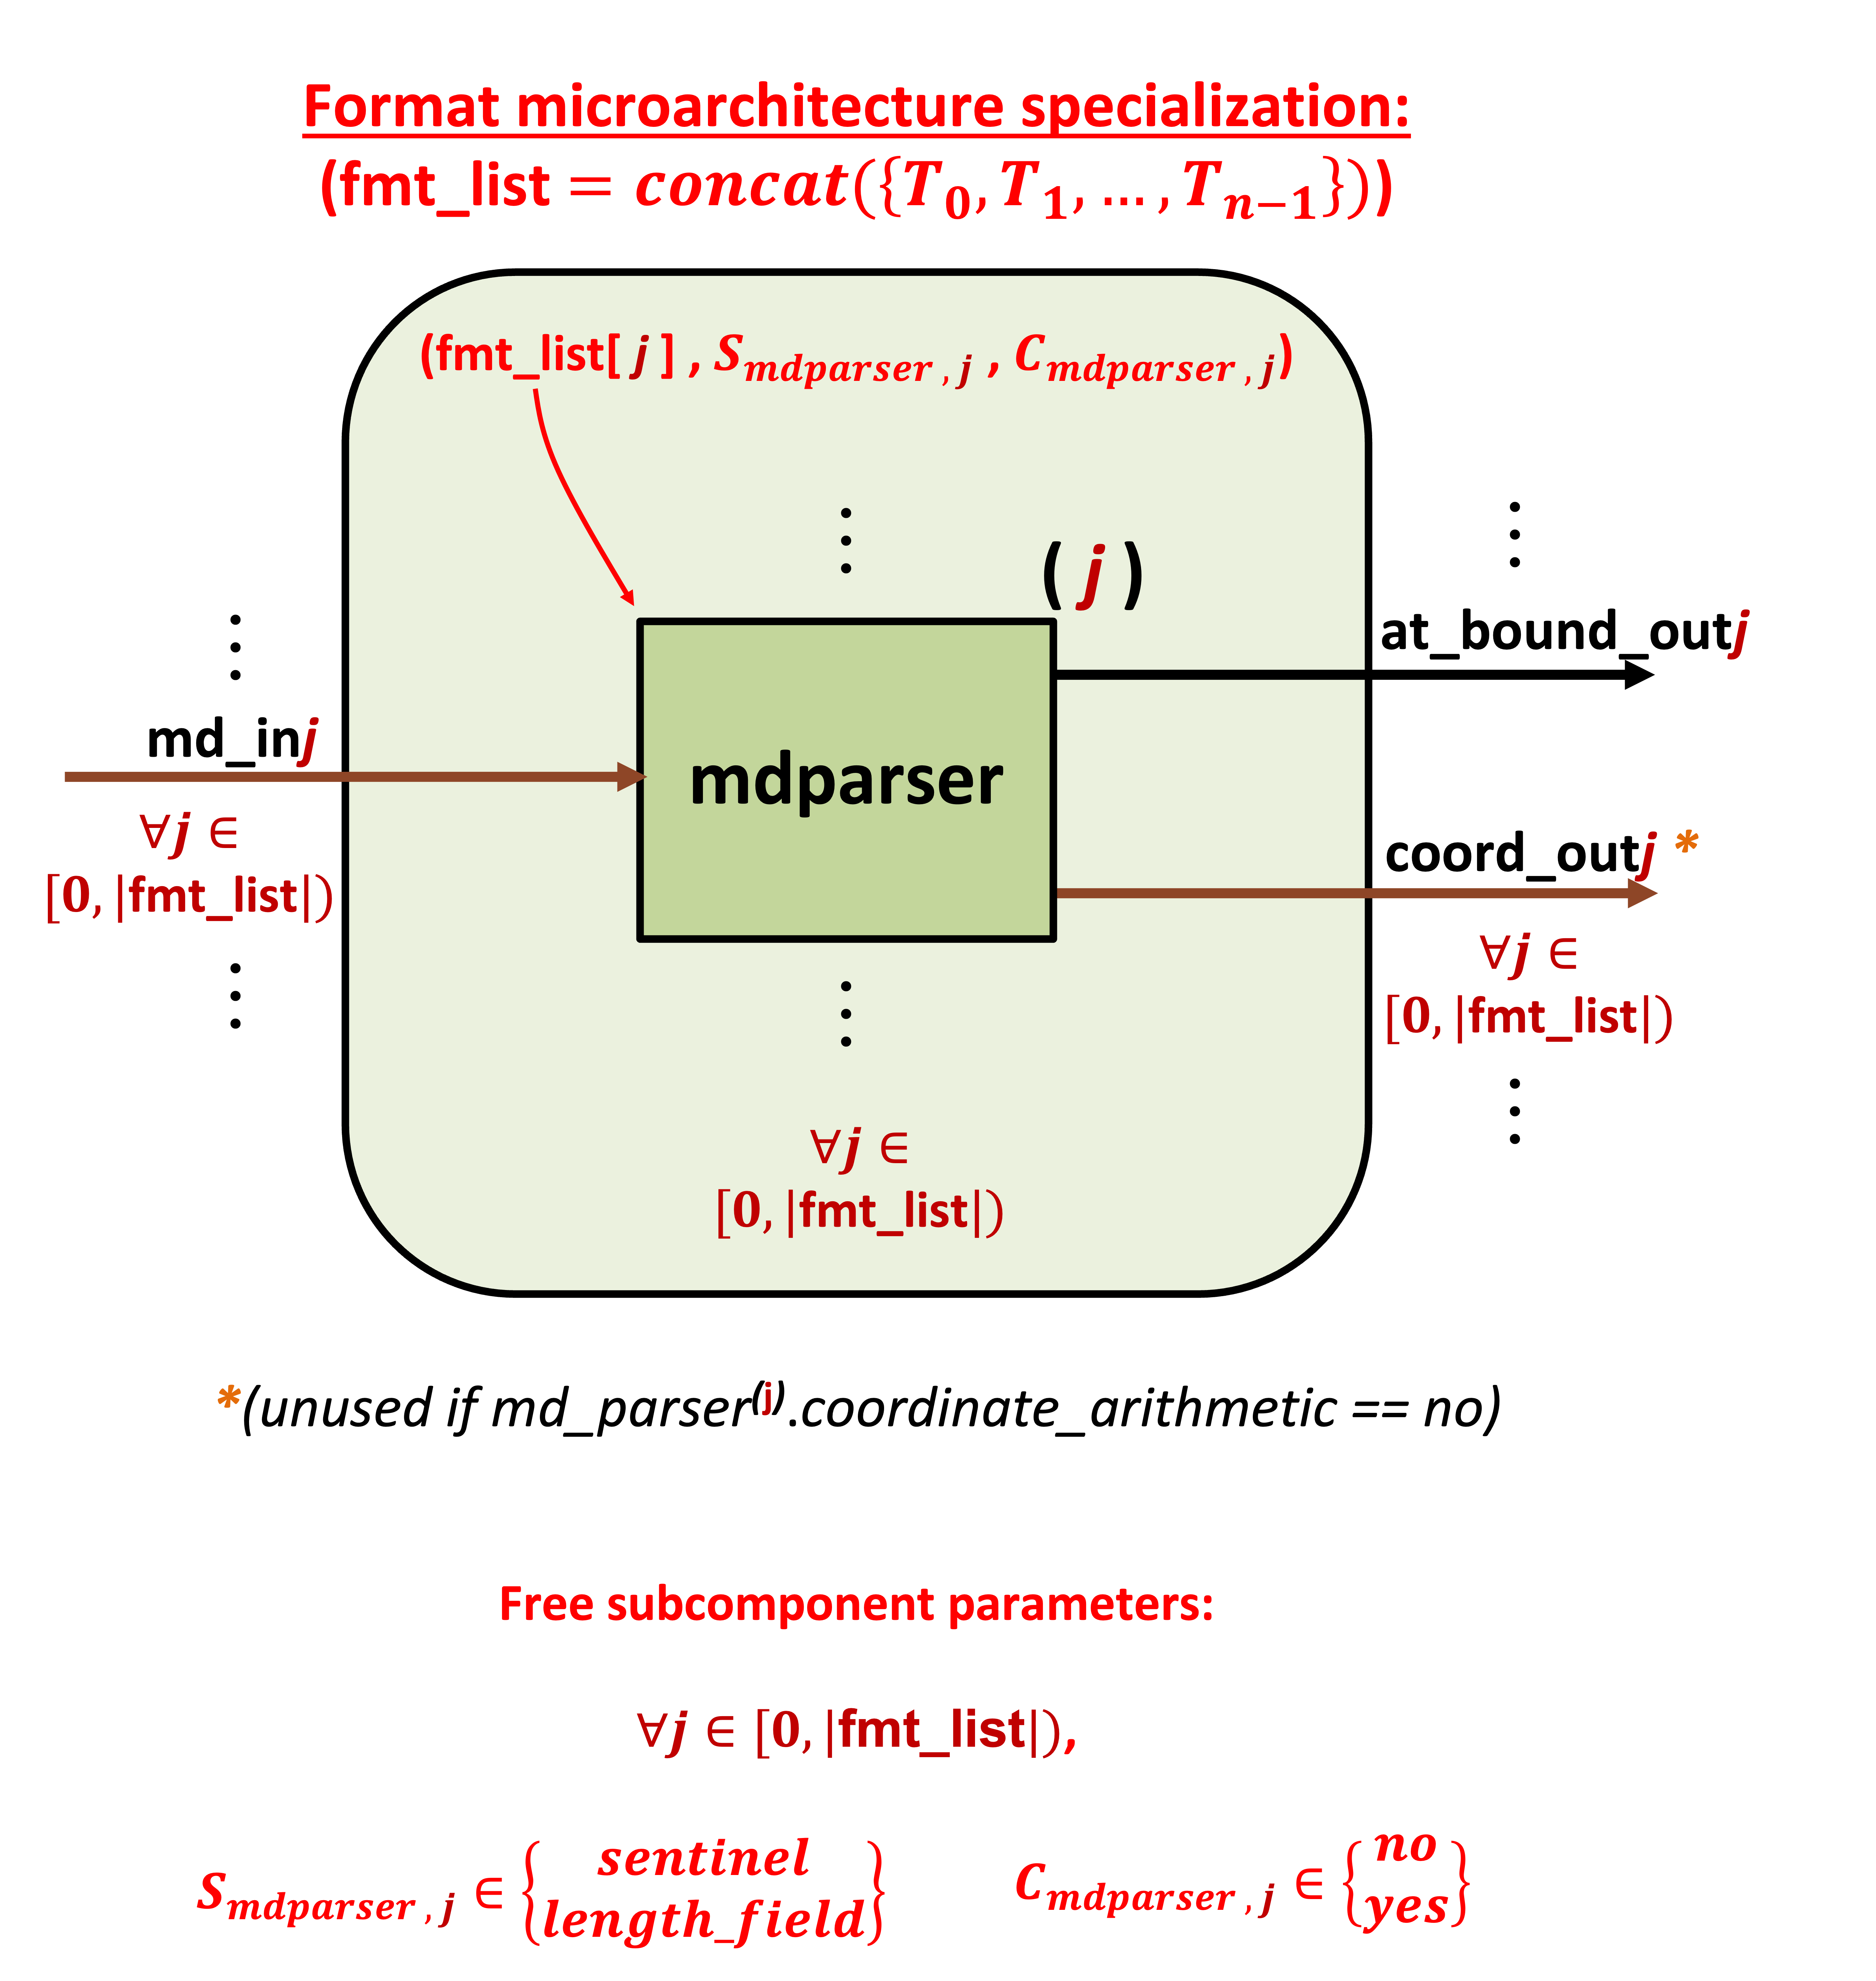
\includegraphics[width=0.95\textwidth]{figures/FMT_all.png}
    \caption{Format microarchitecture implementation topology.}
    \label{fig:FMT_all}
\end{figure}

The FMT block has one attribute - \textit{fmt\_list} - and one supported customization, which covers all possible values of \textit{fmt\_list}. The implementation topology associated with this one customization is shown in Figure~\ref{fig:FMT_all}. The \textit{fmt\_list} attribute is not a free parameter; it is entirely constrained by the sparse representation format of the associated architectural buffer. An architectural buffer keeps\cite{timeloop} one or more dataspaces\cite{timeloop}; if at least one of these dataspaces exploits a format SAF, then the architectural buffer must be associated with a FMT block which parses the sparse format metadata. The \textit{fmt\_list} attribute of the FMT block represents a flattened list of rank formats, for all datatypes resident in the buffer. The  fmt\_list is assumed to have been derived from concatenating the fiber representation regexes\cite{szebook} for all kept dataspaces' fibertrees, excluding dataspaces which do not exploit a format SAF.

As shown in Figure~\ref{fig:FMT_all}, the FMT block contains one or more metadata parsers, one for each sparse rank in the architectural buffer. The \textit{format} attribute of each metadata parser is determined by the format of its corresponding rank. However, as shown in Figure~\ref{fig:FMT_all}, each metadata parser has two free parameters, \textit{sentinel} and \textit{coordinate\_arithmetic}; these are explained in Section~\ref{chapter:primitive_taxo_model}.

%\begin{table}[H]
%\centering
%\begin{tabular}{l}
%\toprule
% fibertree   \\
%\midrule
% *           \\
%\bottomrule
%\end{tabular}
%\caption{Specializations of format microarchitecture}
%\label{tab:format_microarchitecture_specializations}
%\end{table}



\section{Skipping microarchitectures}

\begin{figure}[H]
    \centering
    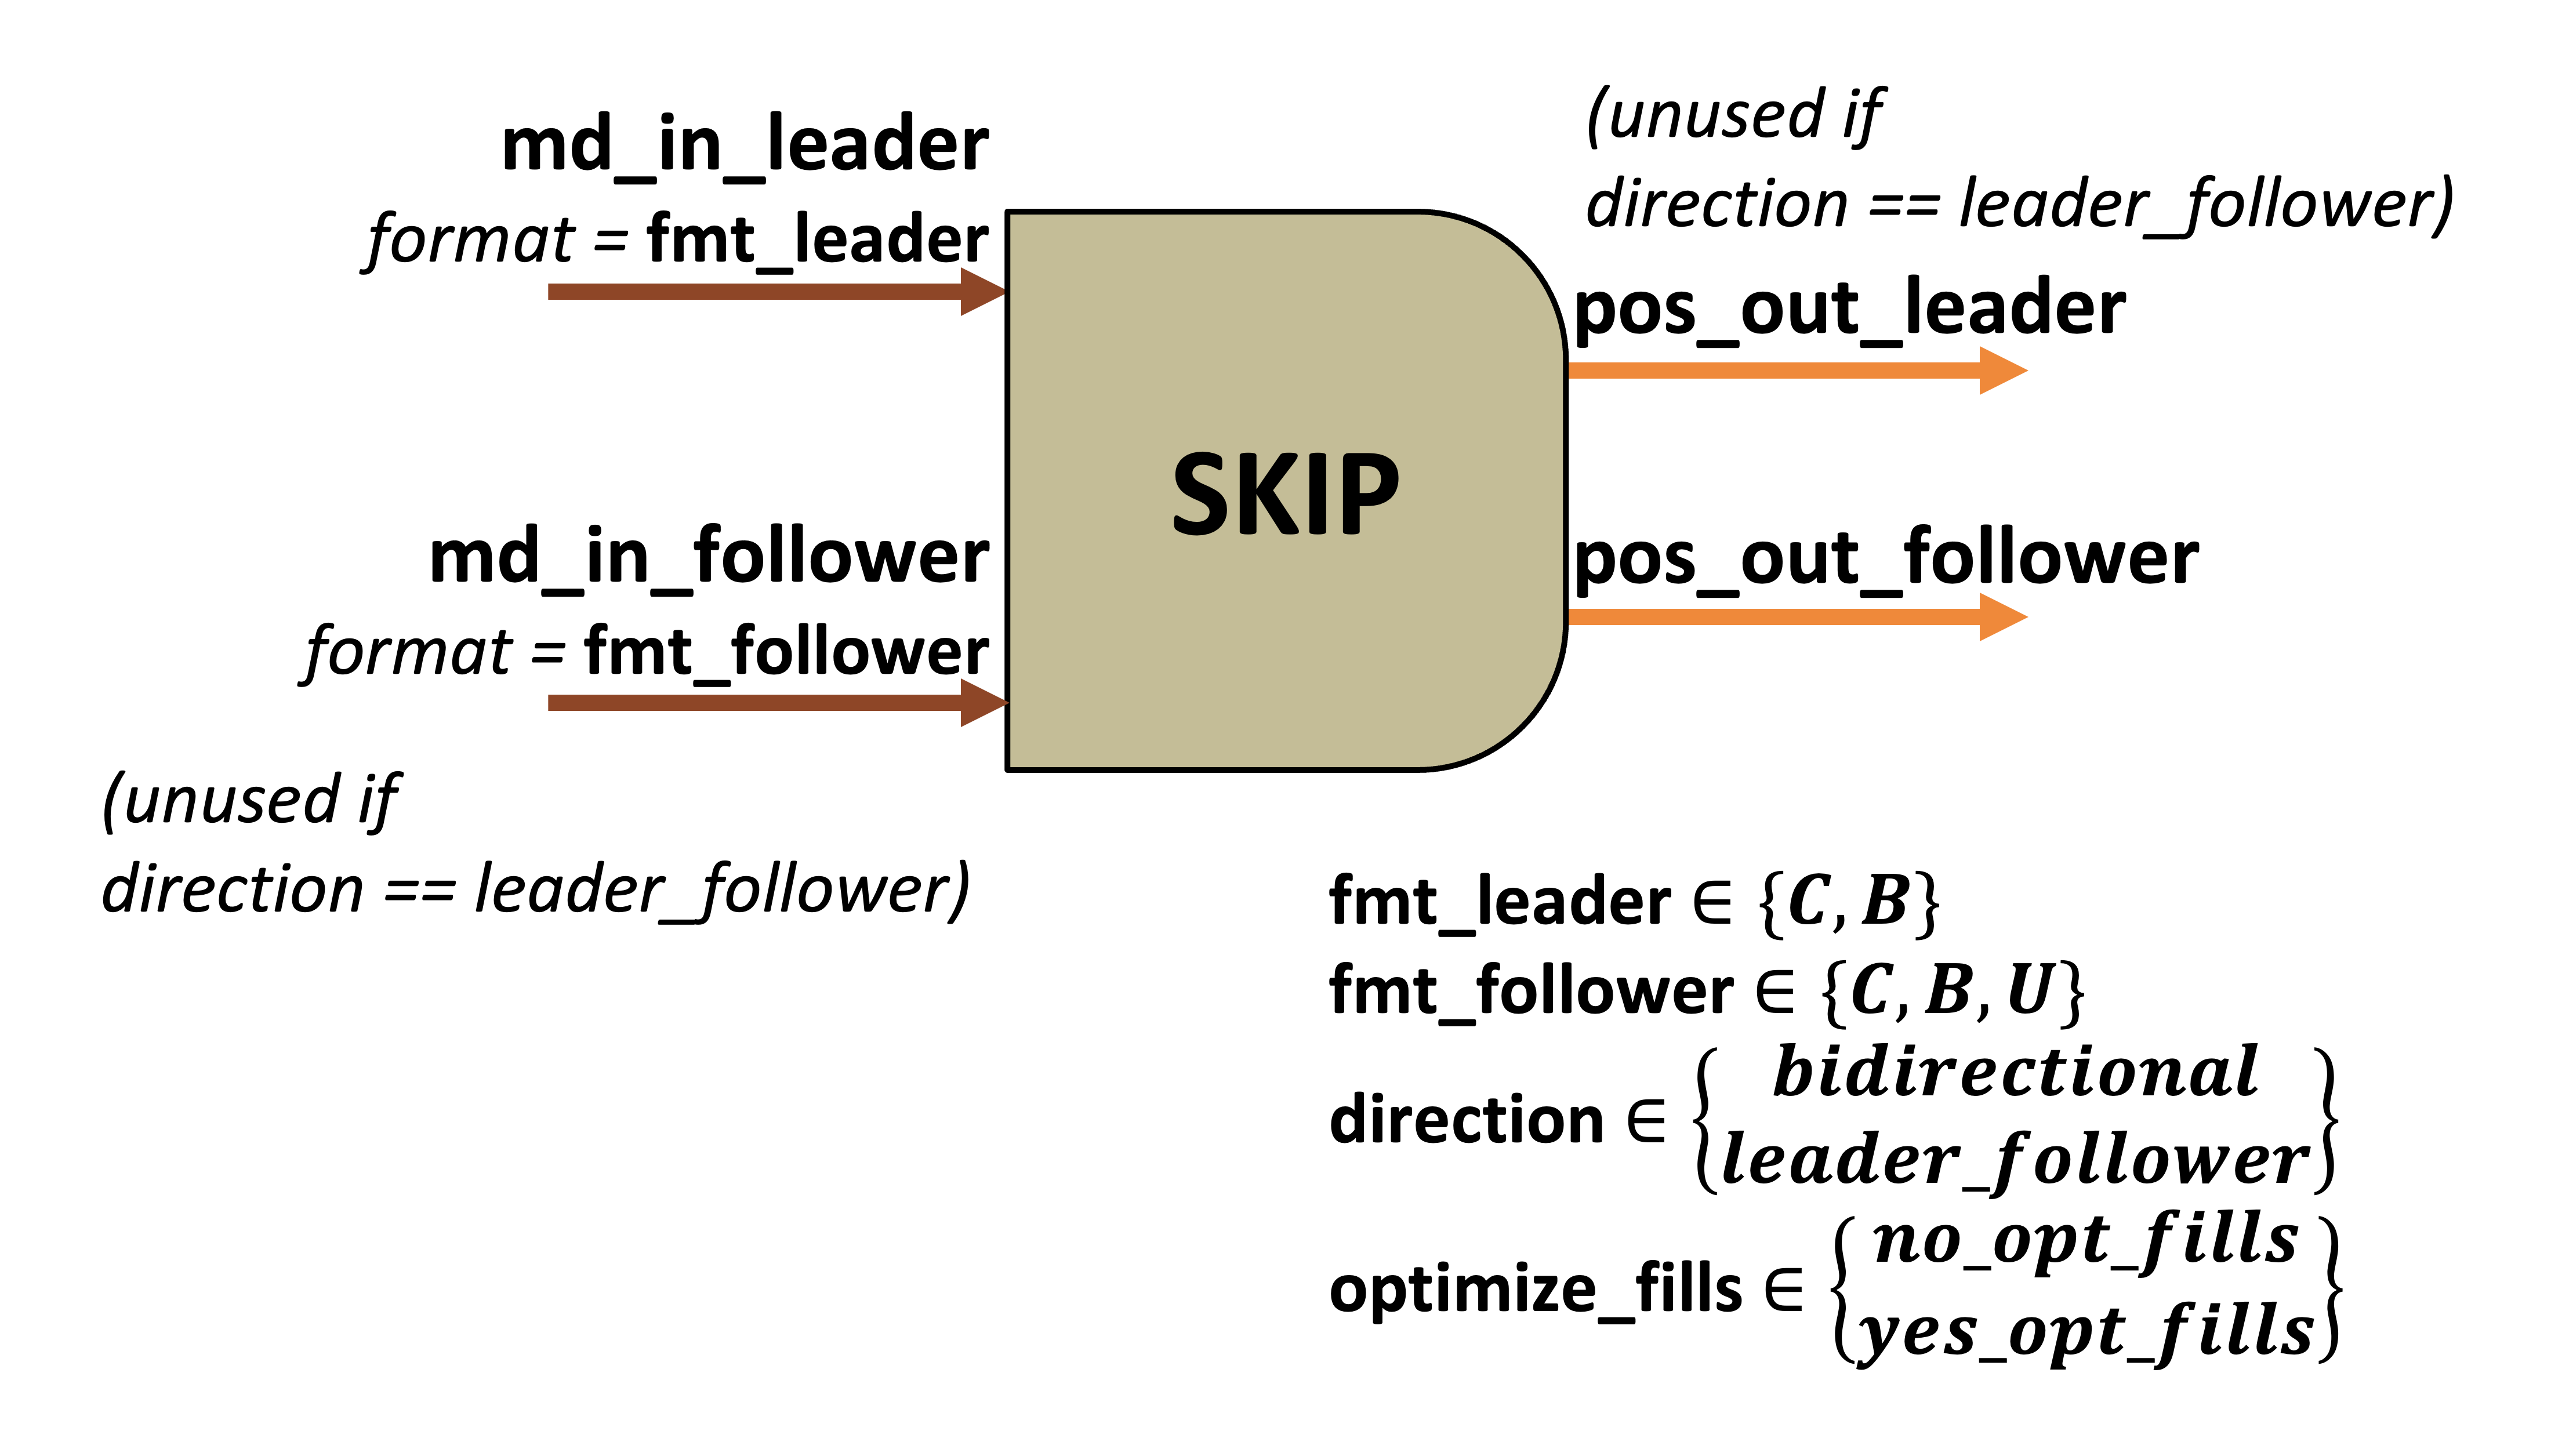
\includegraphics[width=0.95\textwidth]{figures/SKIP.png}
    \caption{Skipping microarchitecture compound component template.}
    \label{fig:SKIP}
\end{figure}

Skipping microarchitectures (SKIP blocks, Figure~\ref{fig:SKIP}) are introduced in Section~\ref{chapter:conceptual_framework}; the function of SKIP blocks is to implement skipping SAFs.

\subsection{Skipping microarchitecture specializations}

\begin{table}[ht]
\centering
\begin{tabular}{llll}
\toprule
 format\_leader   & format\_follower   & direction       & optimize\_fills   \\
\midrule
 C               & C                 & bidirectional   & no\_opt\_fills     \\
 B               & B                 & bidirectional   & no\_opt\_fills     \\
 C               & U                 & leader\_follower & no\_opt\_fills     \\
 C               & U                 & leader\_follower & yes\_opt\_fills    \\
\bottomrule
\end{tabular}
\caption{Specializations of skipping microarchitecture}
\label{tab:Skipping microarchitecture_specializations}
\end{table}

The supported SKIP block customizations can be found in Table~\ref{tab:Skipping microarchitecture_specializations}.

\begin{figure}[H]
    \centering
    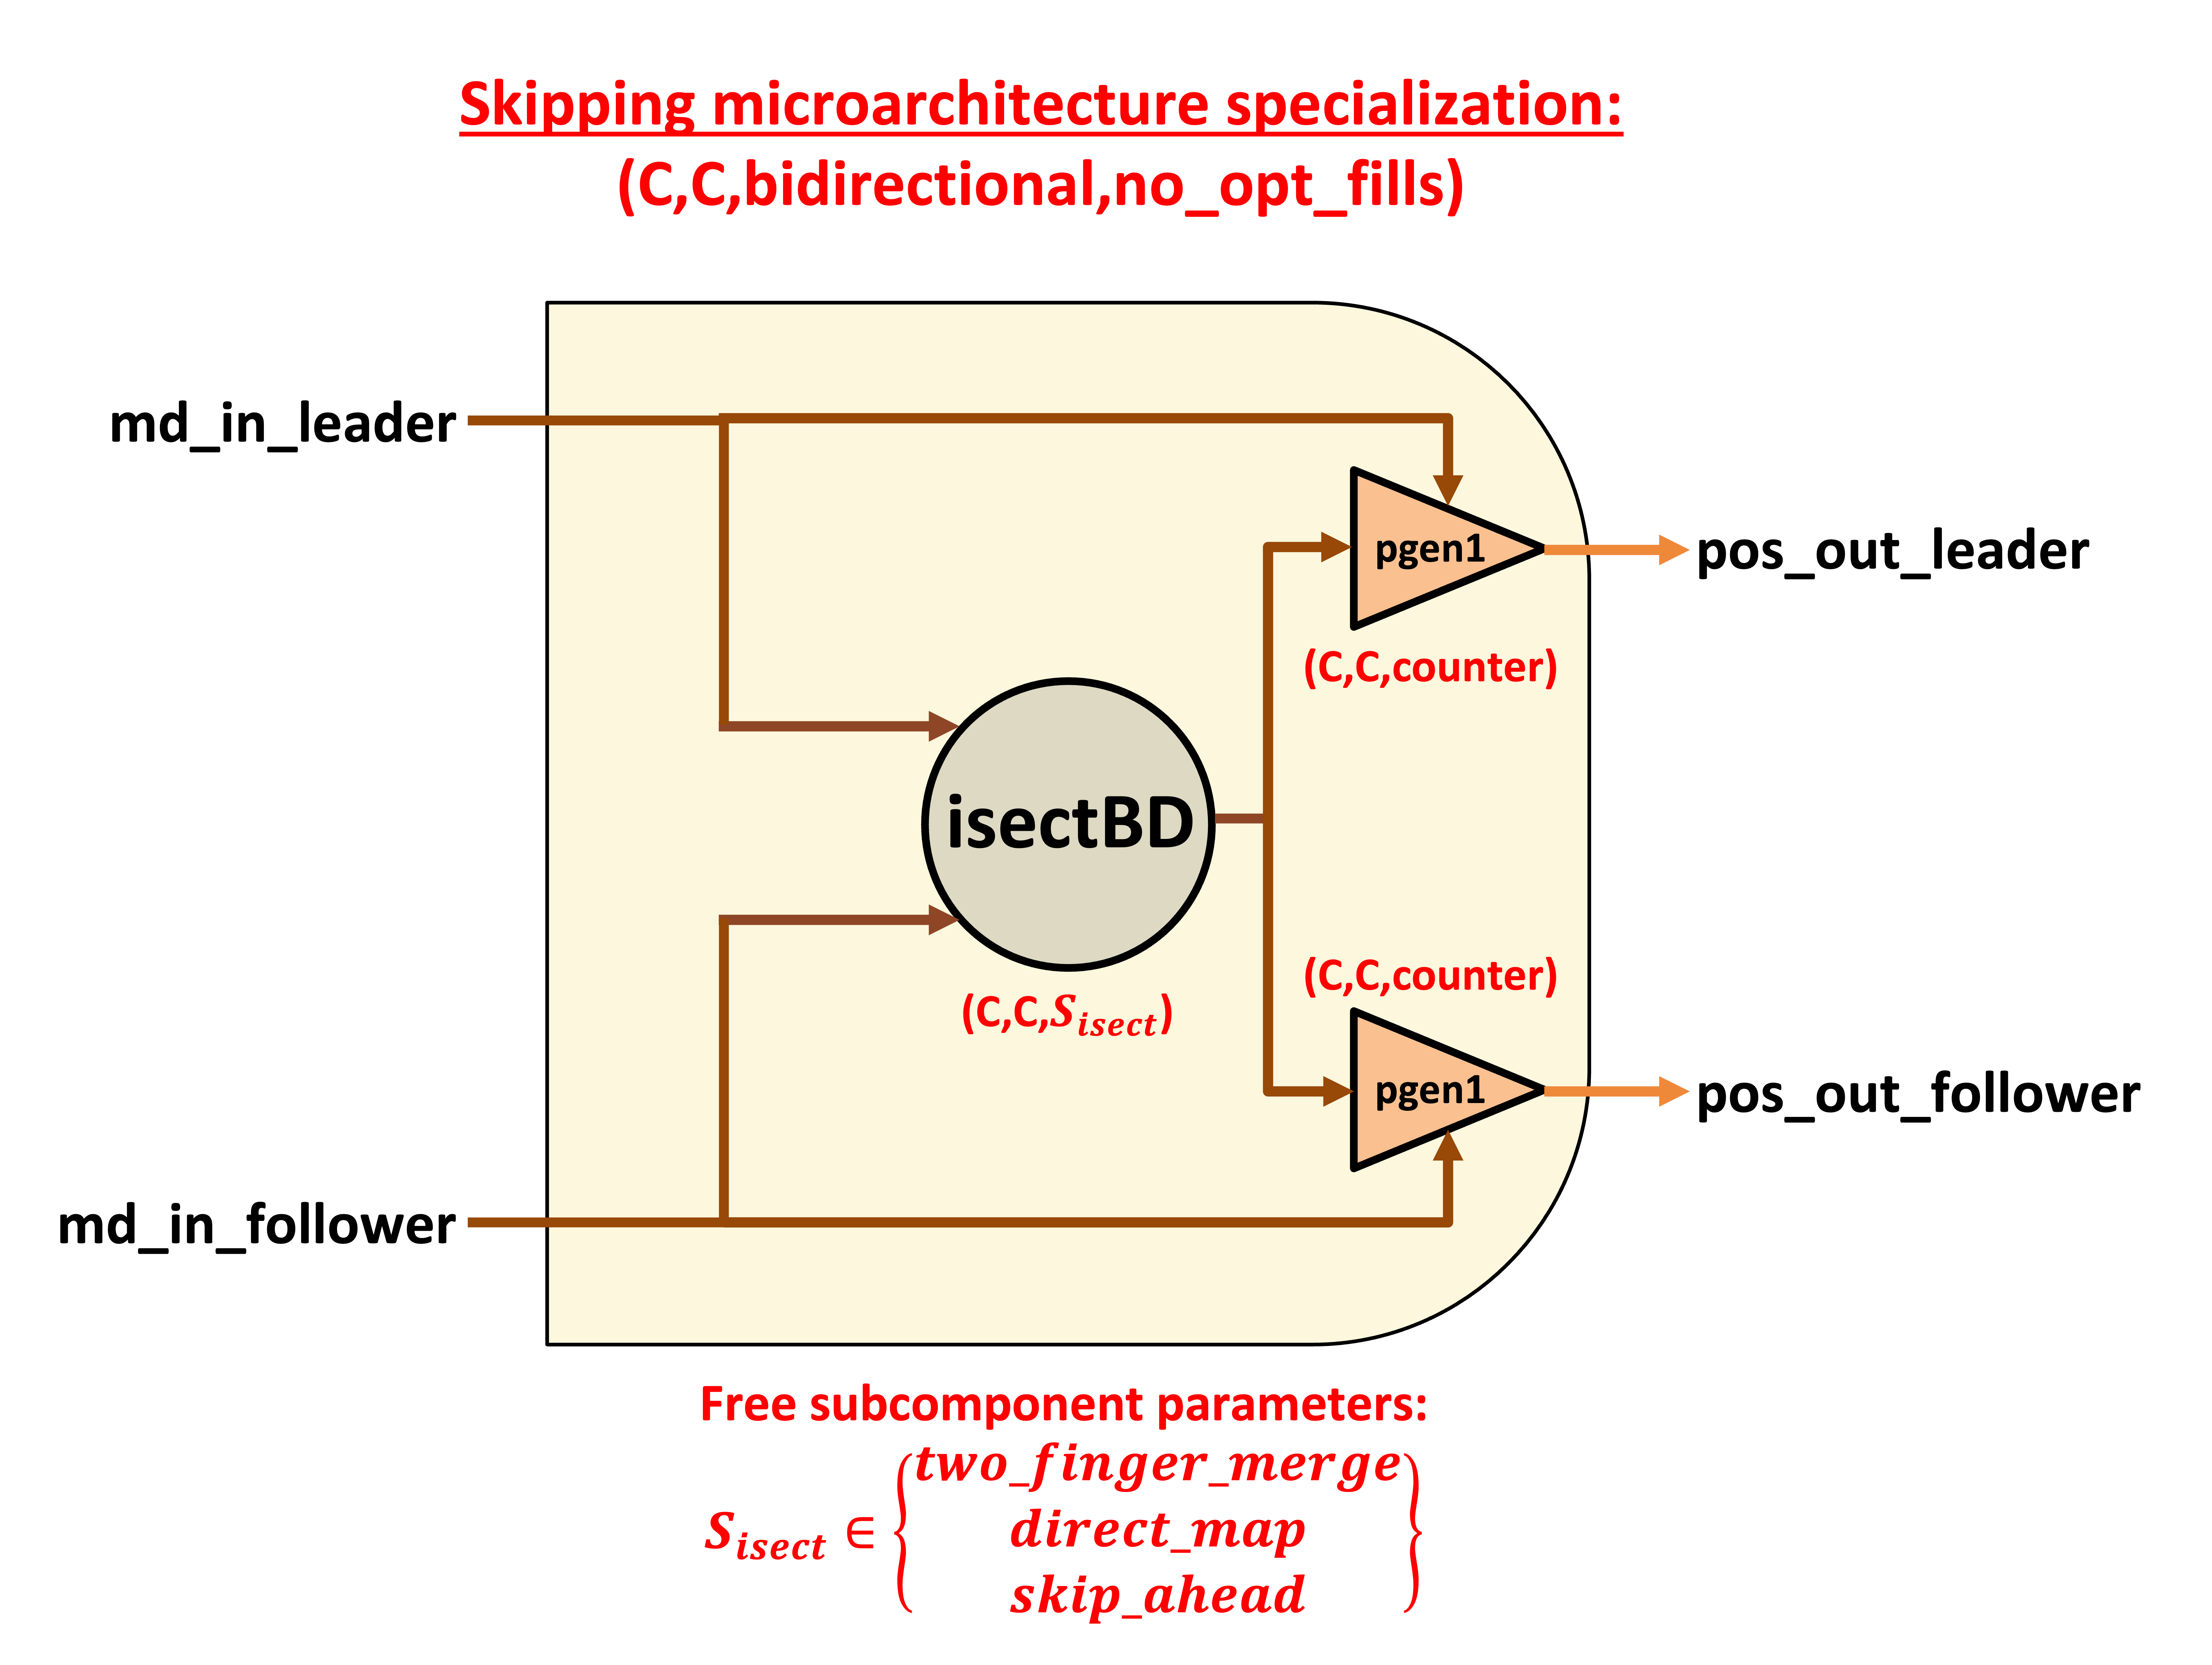
\includegraphics[width=0.95\textwidth]{figures/SKIP_C_C_bidirectional_no_opt_fills.png}
    \caption{Bidirectional coordinate-payload (C) skipping microarchitecture implementation topology (``ExTensor-like''\cite{extensor}.)}
    \label{fig:SKIP_C_C_bidirectional_no_opt_fills}
\end{figure}

\begin{figure}[H]
    \centering
    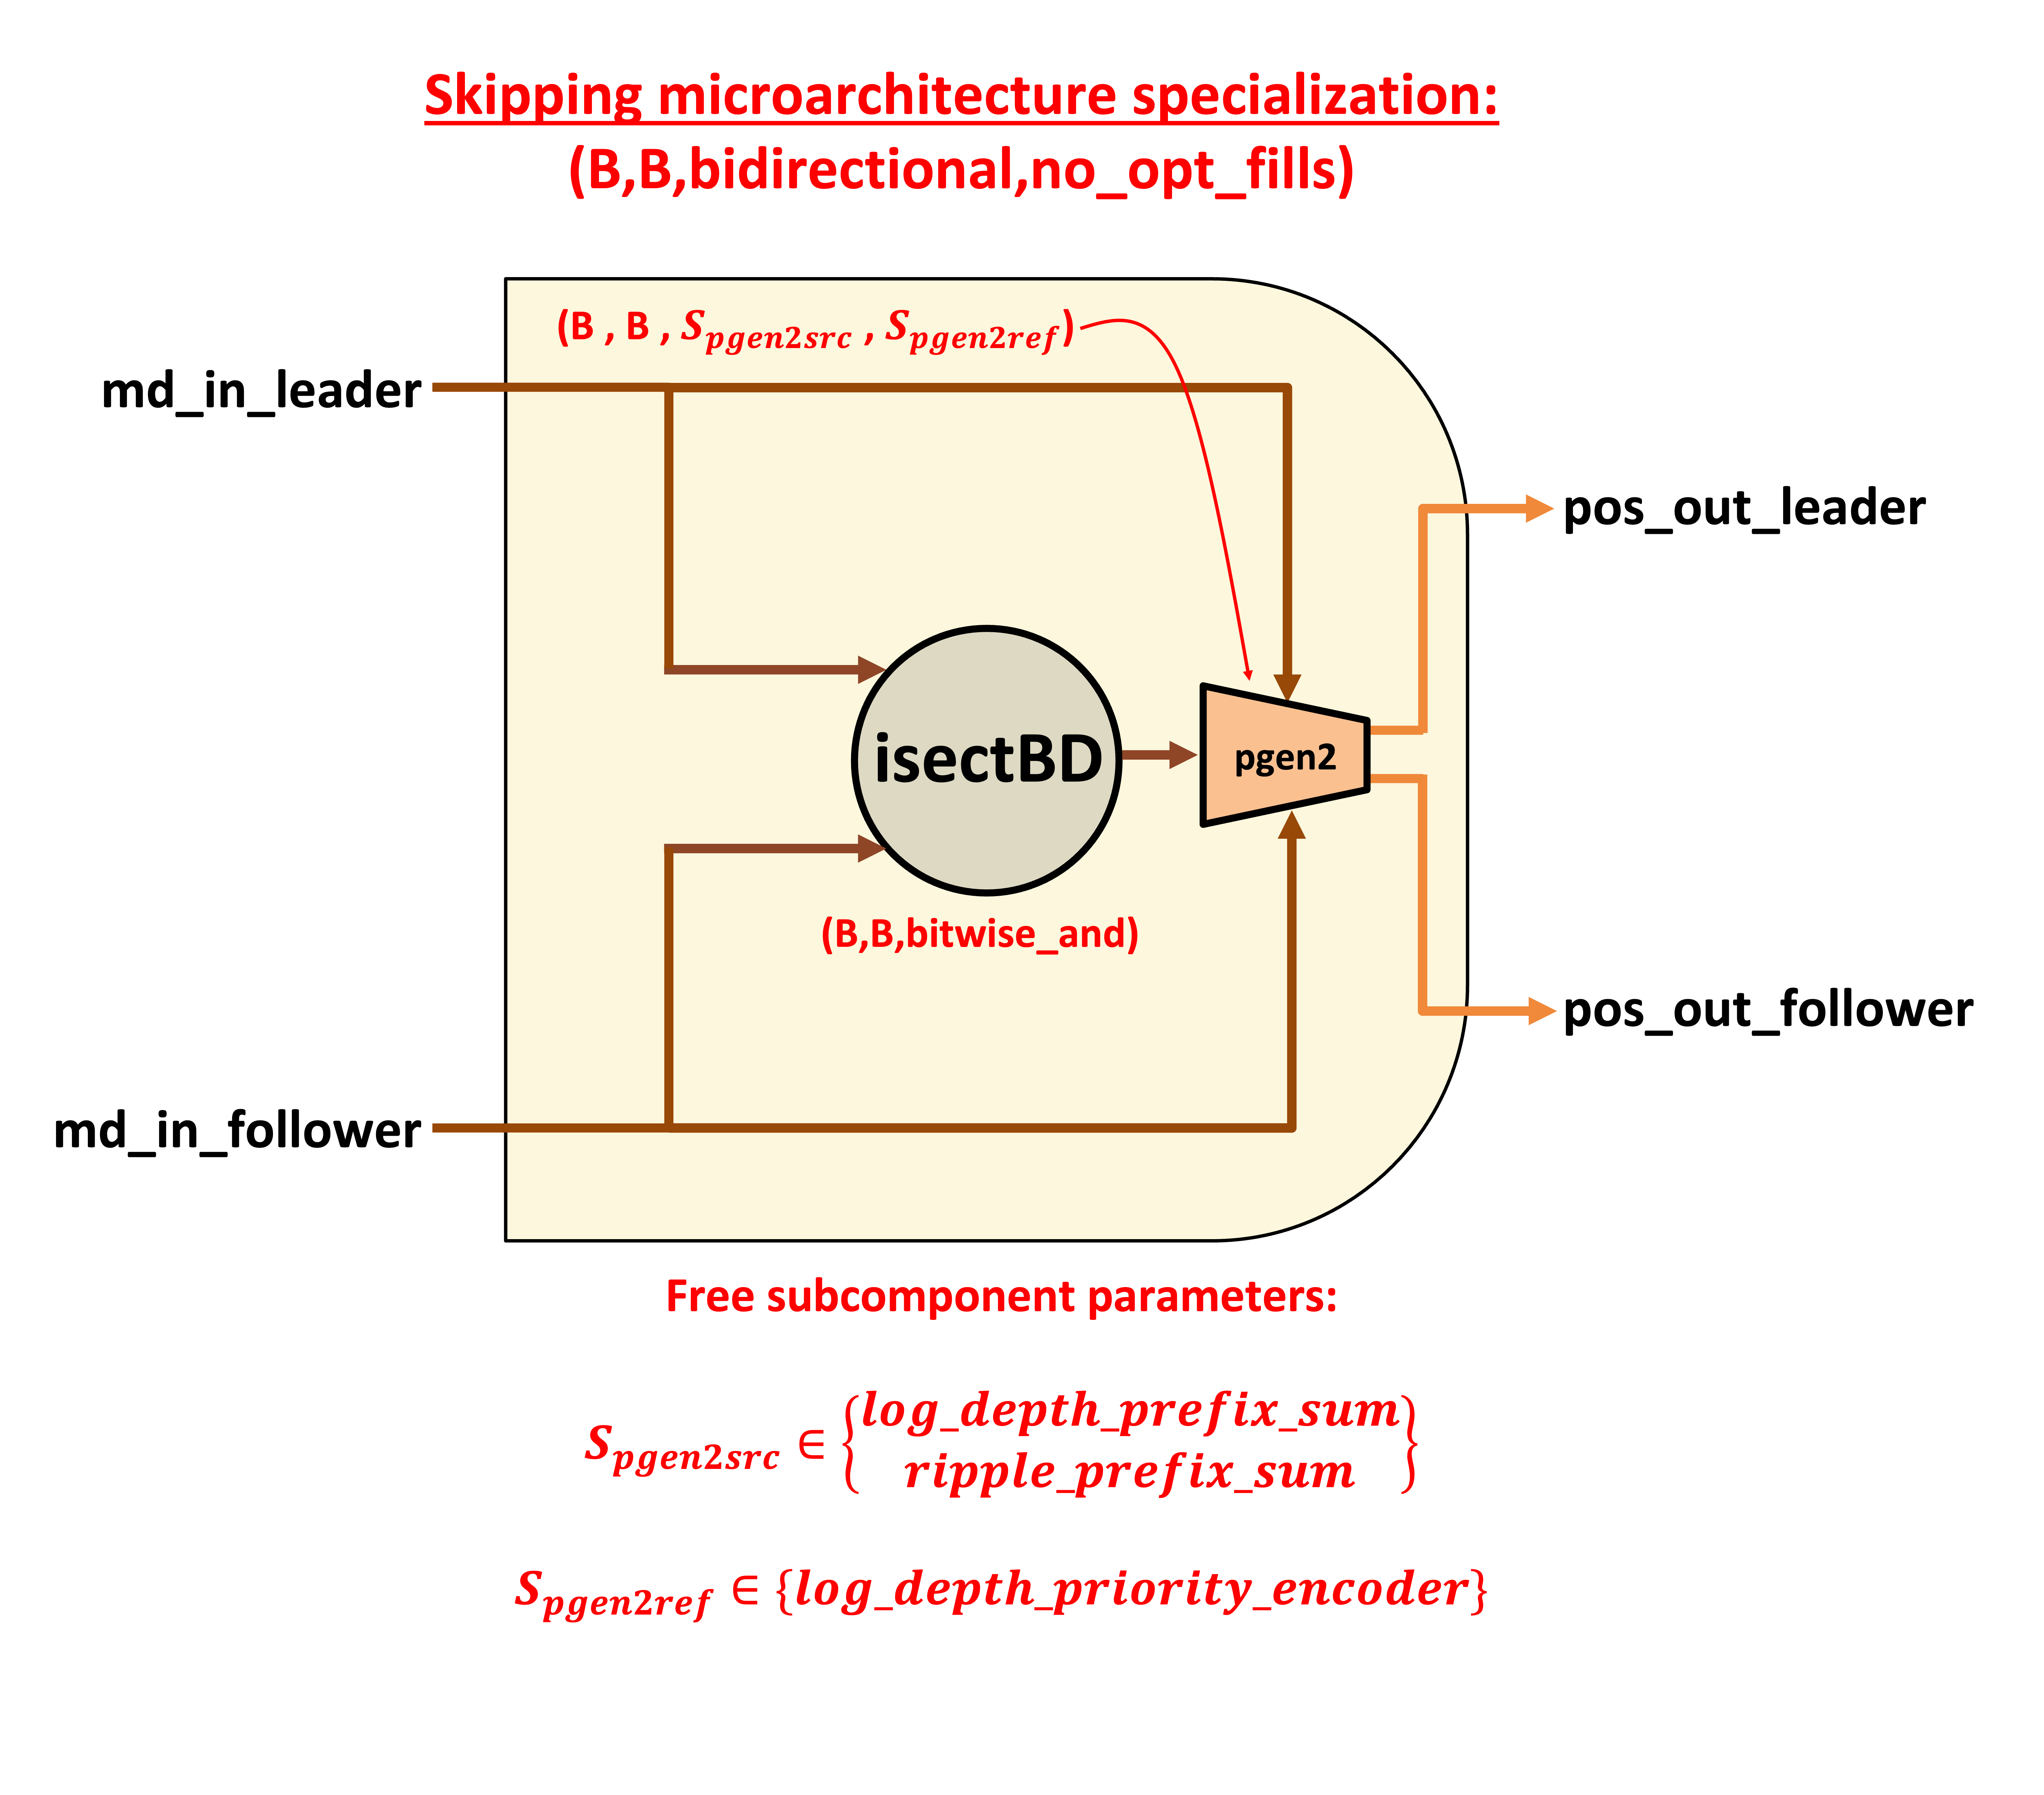
\includegraphics[width=0.95\textwidth]{figures/SKIP_B_B_bidirectional_no_opt_fills.png}
    \caption{Bidirectional bitmask (B) skipping microarchitecture implementation topology (``SparTen-like''\cite{sparten}.)}
    \label{fig:SKIP_B_B_bidirectional_no_opt_fills}
\end{figure}

Figure~\ref{fig:SKIP_C_C_bidirectional_no_opt_fills} shows the implementation topology of the ExTensor-like\cite{extensor} bidirectional coordinate-payload skipping microarchitecture; Figure~\ref{fig:SKIP_B_B_bidirectional_no_opt_fills} shows the implementation topology of the SparTen-like\cite{sparten} bidirectional bitmask skipping microarchitecture. These two implementation topologies were introduced in Section~\ref{chapter:conceptual_framework}.

The bidirectional coordinate-payload skipping microarchitecture has one free parameter, $S_{isect}$, which is the \textit{strategy} attribute of the underlying bidirectional intersection unit. It has three supported values, corresponding to two-fingered merge, direct-mapped intersection unit, and skip-ahead intersection unit; these options are discussed in Section~\ref{chapter:primitive_taxo_model}.

The bidirectional bitmask skipping microarchitecture has two free parameters, $S_{pgen2src}$ and $S_{pgen2ref}$:

\[ S_{pgen2src} \in (log\_depth\_prefix\_sum , ripple\_prefix\_sum) \]

\[ S_{pgen2ref} \in (log\_depth\_priority\_encoder) \]

\begin{figure}[H]
    \centering
    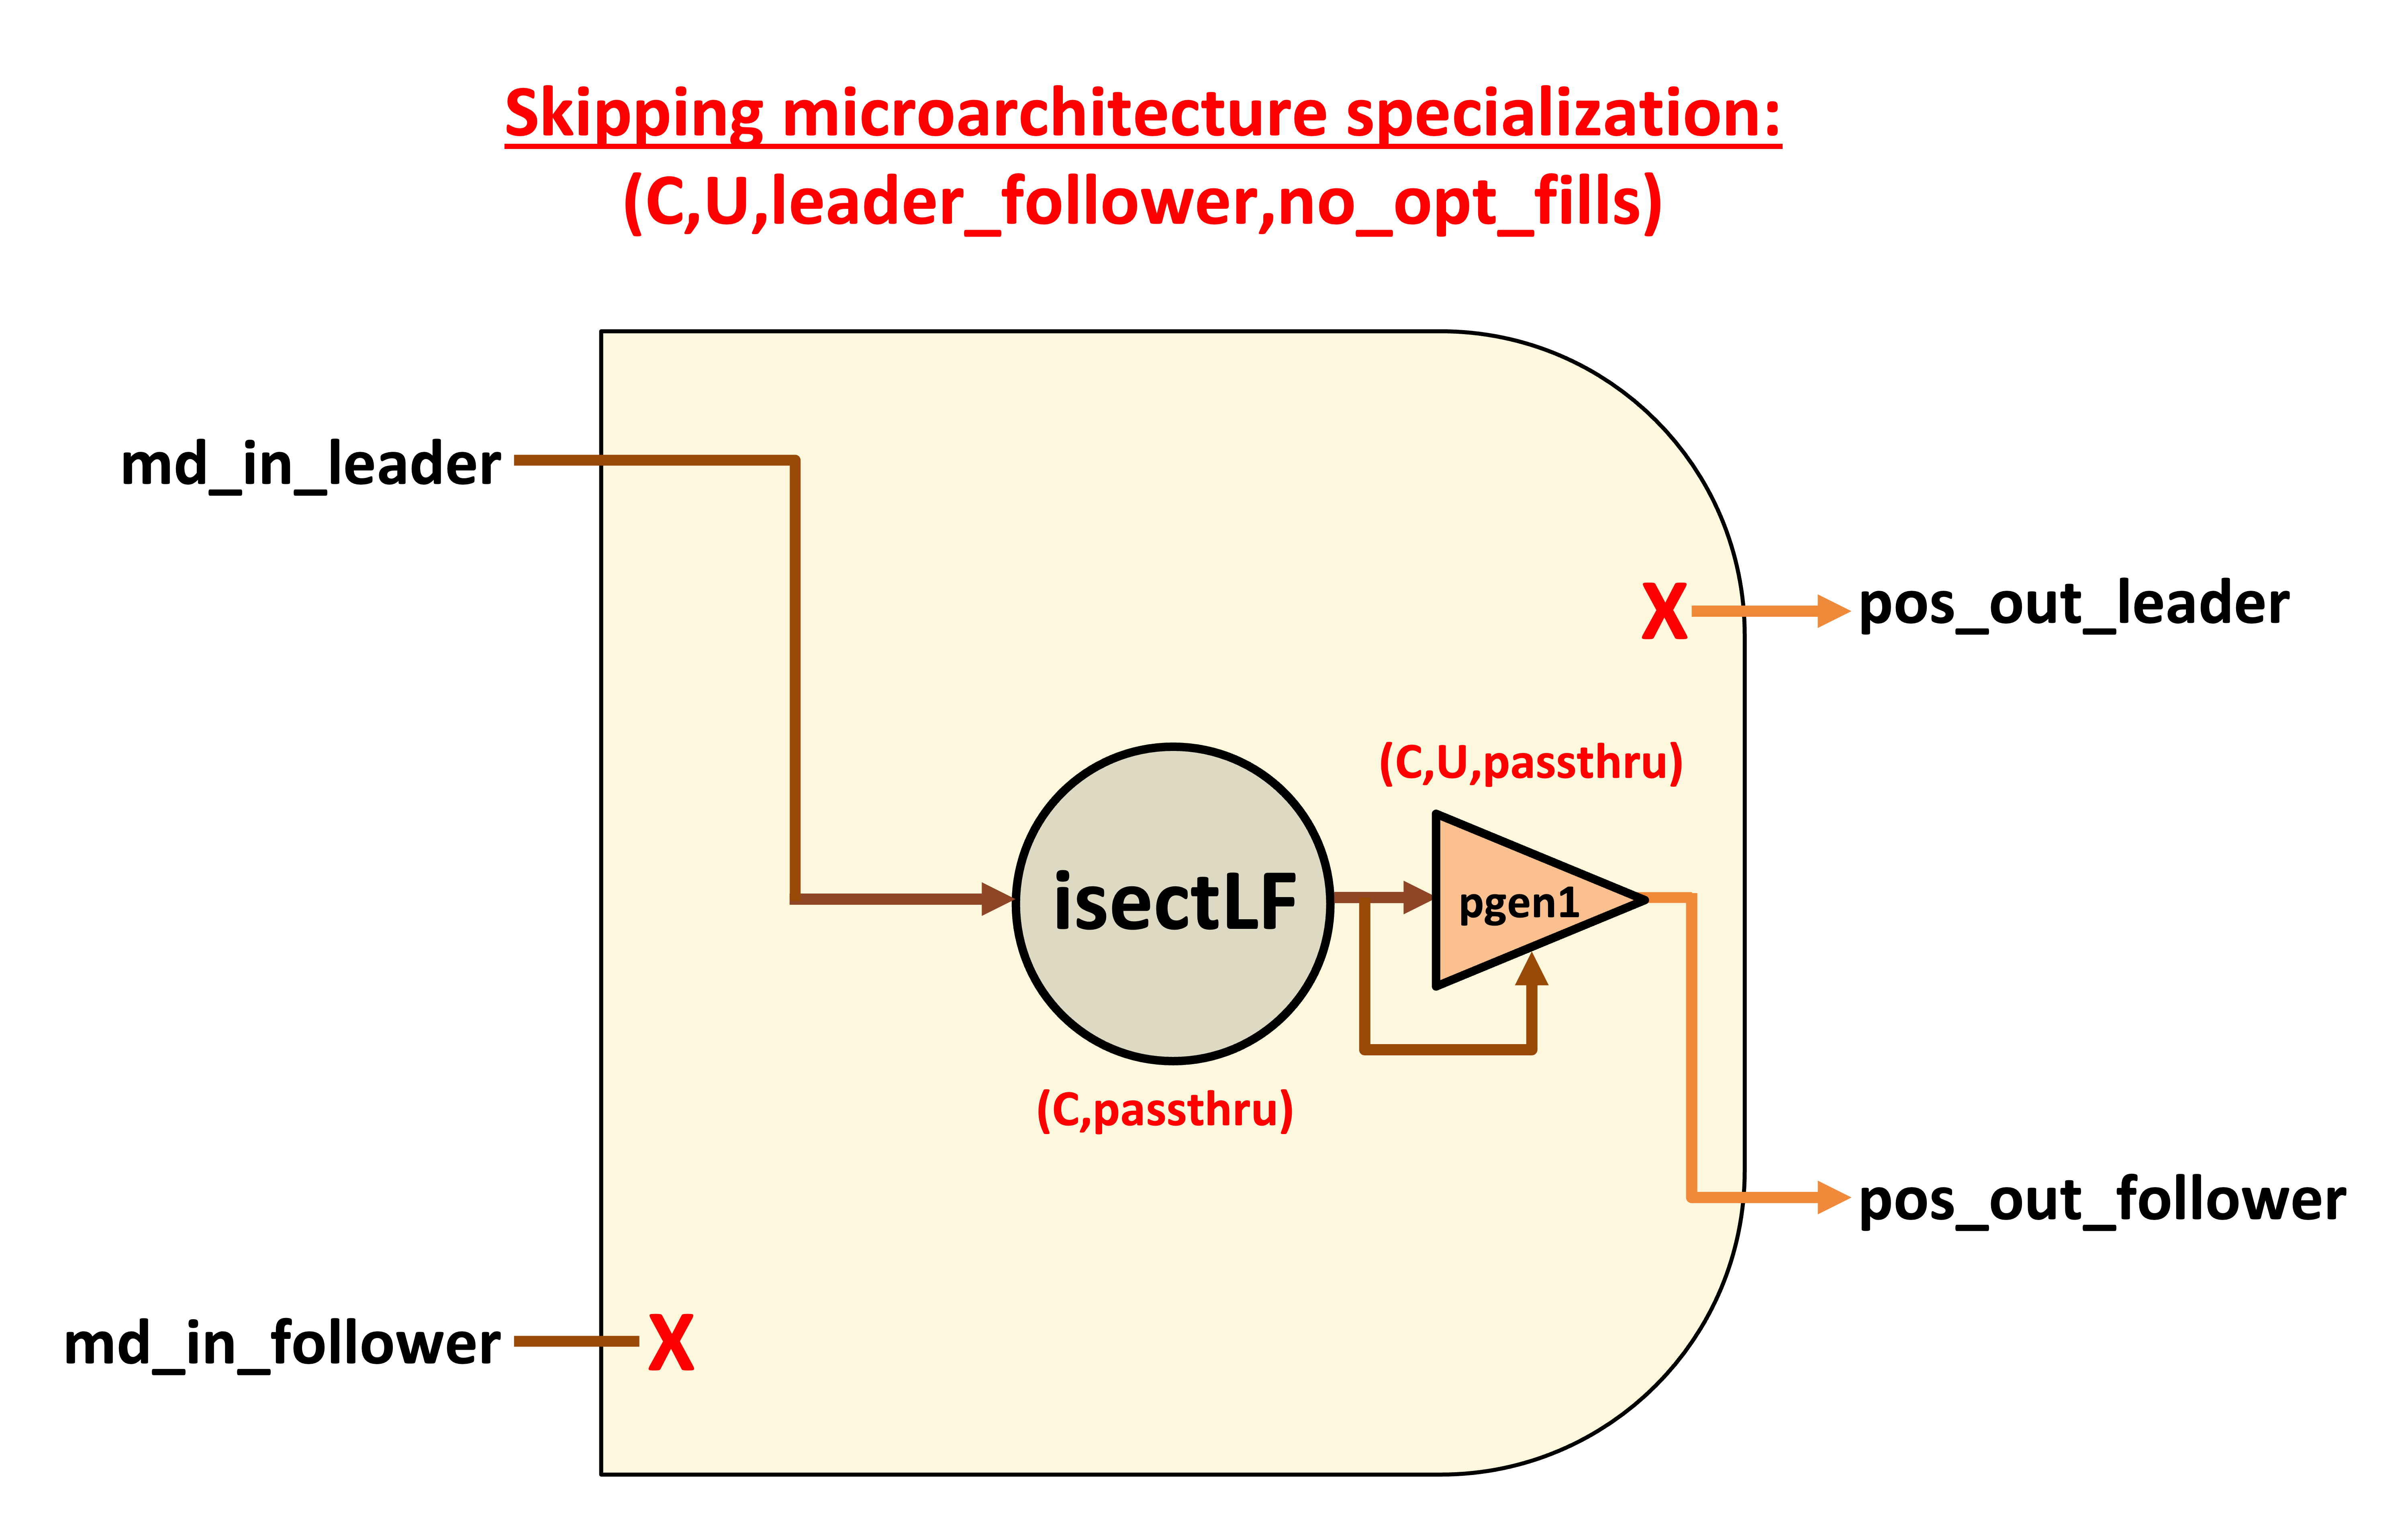
\includegraphics[width=0.95\textwidth]{figures/SKIP_C_U_leader_follower_no_opt_fills.png}
    \caption{Leader-follower coordinate-payload (C) to uncompressed offset-pair (U) skipping microarchitecture implementation topology, without fill optimization.}
    \label{fig:SKIP_C_U_leader_follower_no_opt_fills}
\end{figure}

\begin{figure}[H]
    \centering
    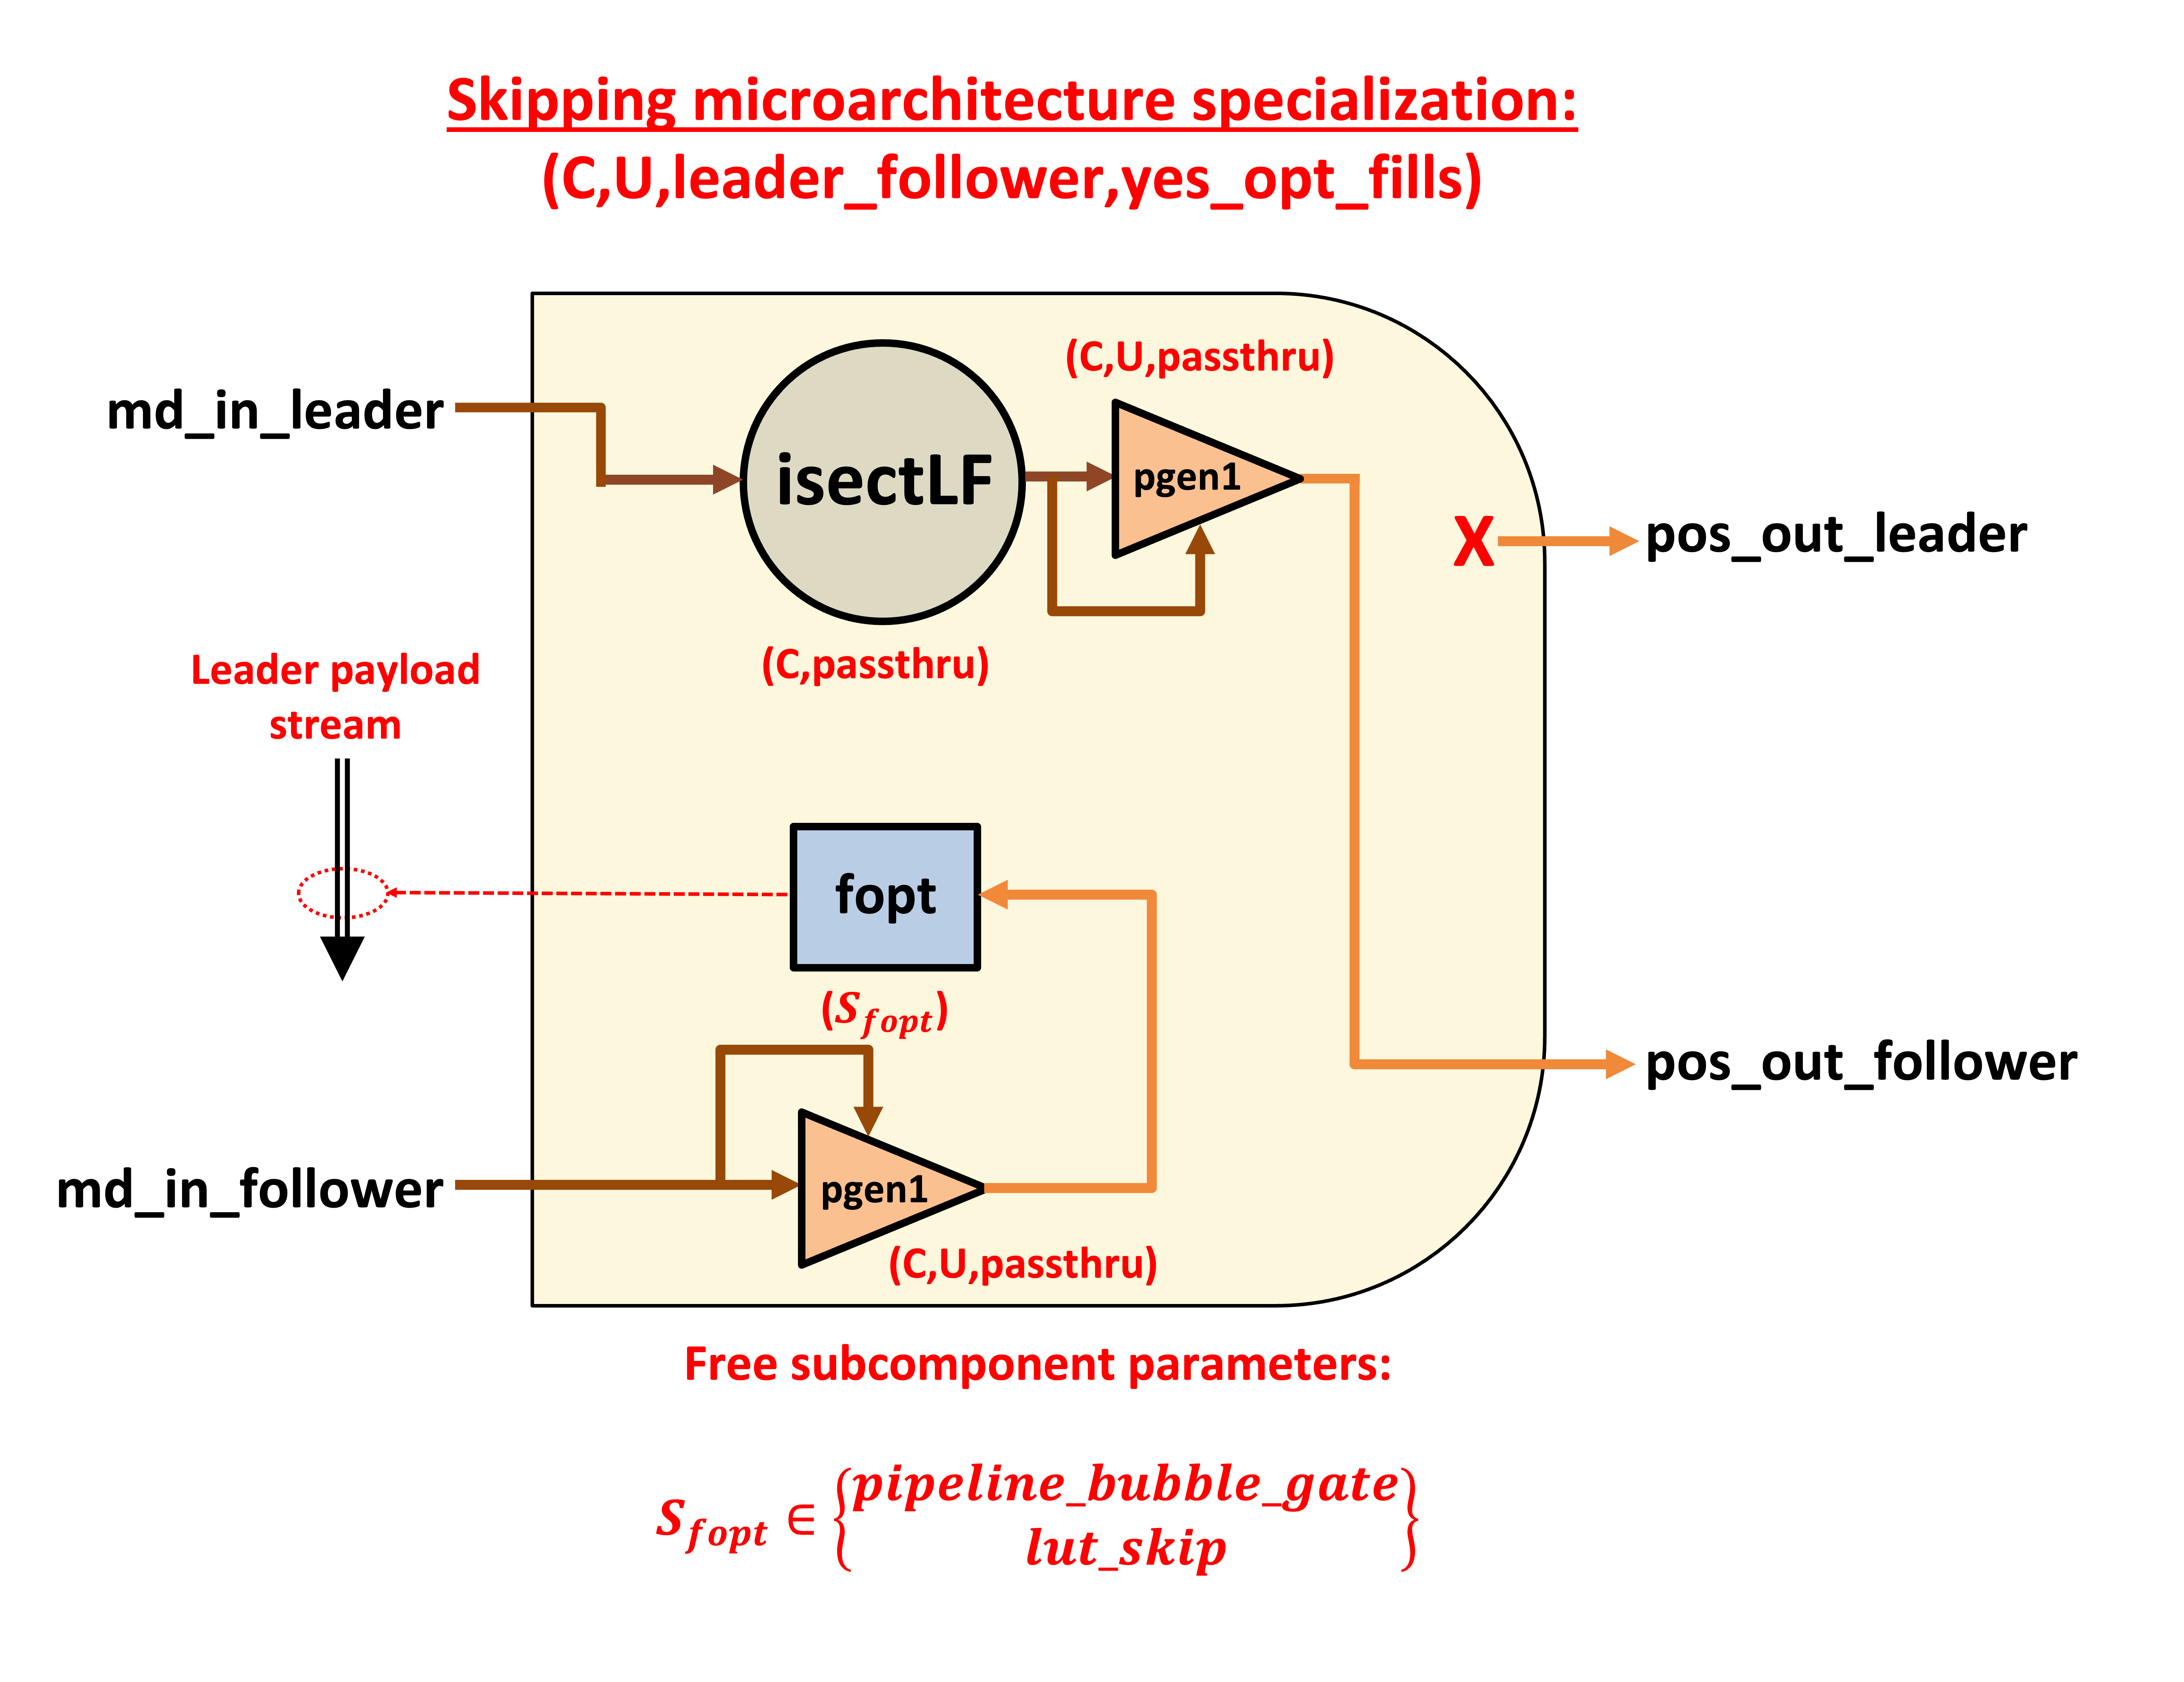
\includegraphics[width=0.95\textwidth]{figures/SKIP_C_U_leader_follower_yes_opt_fills.png}
    \caption{Leader-follower coordinate-payload (C) to uncompressed offset-pair (U) skipping microarchitecture implementation topology, with fill optimization (``Eyeriss-v2-like''\cite{eyerissv2}.)}
    \label{fig:SKIP_C_U_leader_follower_yes_opt_fills}
\end{figure}

Figures~\ref{fig:SKIP_C_U_leader_follower_yes_opt_fills} and~\ref{fig:SKIP_C_U_leader_follower_no_opt_fills} compare coordinate-payload leader-follower skipping microarchitectures, with and without fill optimization. The variant with fill optimization has one free parameter, $S_{fopt}$:

\[S_{fopt} \in (pipeline\_bubble\_skip,lut\_skip)\]

These are the choices of the fill optimizer \textit{strategy} attribute, which is discussed in Section~\ref{chapter:primitive_taxo_model}.

%\section{SAF concretization}
%\label{chapter:saf_concretization}